\section{講義概要}


\begin{frame}
\frametitle{今日の内容}



\begin{enumerate}
\item ロピタルの定理
\item ロルの定理, 平均値の定理, コーシーの平均値の定理, 
\item 高次導関数, テイラーの定理, 有限テイラー展開
\end{enumerate} 



\end{frame}


\section{ロピタルの定理}

\begin{frame}
\frametitle{ロピタルの定理(L'Hopital's theorem)}

微分は不定形の極限を計算する強力な手法を与える. 

\begin{Thm}[ロピタルの定理]
関数$f(x),g(x)$が$a$を除く$a$の近傍において微分可能であり, 
$$
\lim_{x\to a}f(x) = \lim_{x\to a}g(x)=0
$$
かつ$g'(x) \ne0$とする. このとき極限$\displaystyle \lim_{x\to a}\frac{f'(x)}{g'(x)}$が存在するならば
$$
\lim_{x\to a}\frac{f(x)}{g(x)} = \lim_{x\to a}\frac{f'(x)}{g'(x)}. 
$$
\end{Thm}

ロピタルの定理は$a=\pm \infty$や$\displaystyle \lim_{x\to a}f(x) = \lim_{x\to a}g(x)=\pm \infty$の場合にも成立する. 
証明は次回行う. 

\end{frame}


%%%%%%%%%%%%%%%%%%%%%%%%%%%%%%%%%%%%%%%%%%%%%%%%%%%%%%%%%%%%%%%%%%%%%%%%%%%%%%%%%%%%%%%
%%%%%%%%%%%%%%%%%%%%%%%%%%%%%%%%%%%%%%%%%%%%%%%%%%%%%%%%%%%%%%%%%%%%%%%%%%%%%%%%%%%%%%%


\begin{frame}
\frametitle{ロピタルの定理}


\begin{Prob}
次の極限を計算せよ. ロピタルの定理を使う際には, 仮定に注意する.  \vspace{2mm}
\begin{enumerate}
\item $\displaystyle \lim_{x\to 0} \frac{\sin x}{x}$ \vspace{2mm}
\item  $\displaystyle \lim_{x\to 1} \frac{\log x}{x-1}$ \vspace{2mm}
\item $\displaystyle \lim_{x\to \infty} \frac{10^{10}x}{e^x}$ \vspace{2mm}
\item $\displaystyle \lim_{x\to 0} \frac{\sqrt{x+1}-1}{x}$ \vspace{2mm}
\item $\displaystyle \lim_{x\to 0} \frac{\sin x-x}{x^3}$ 
\end{enumerate}
\end{Prob}

\end{frame}

%%%%%%%%%%%%%%%%%%%%%%%%%%%%%%%%%%%%%%%%%%%%%%%%%%%%%%%%%%%%%%%%%%%%%%%%%%%%%%%%%%%%%%%
%%%%%%%%%%%%%%%%%%%%%%%%%%%%%%%%%%%%%%%%%%%%%%%%%%%%%%%%%%%%%%%%%%%%%%%%%%%%%%%%%%%%%%%


\begin{frame}
\frametitle{ロピタルの定理}

答え

\begin{enumerate}
\item $\displaystyle \lim_{x\to 0} \frac{\sin x}{x}= \lim_{x\to 0} \frac{\cos x}{1}=1$ \vspace{3mm}
\item  $\displaystyle \lim_{x\to 1} \frac{\log x}{x-1}= \lim_{x\to 1} \frac{x^{-1}}{1}=1$ \vspace{3mm}
\item $\displaystyle \lim_{x\to \infty} \frac{10^{10}x}{e^x}= \lim_{x\to \infty} \frac{10^{10}}{e^x}=0$ \vspace{3mm}
\item $\displaystyle \lim_{x\to 0} \frac{\sqrt{x+1}-1}{x}= \lim_{x\to 0} \frac{\frac{1}{2}(x+1)^{-\frac{1}{2}}}{1}=\frac{1}{2}$ \vspace{3mm}
\item $\displaystyle \lim_{x\to 0} \frac{\sin x-x}{x^3}= \lim_{x\to 0} \frac{\cos x-1}{3x^2}= \lim_{x\to 0} \frac{-\sin x}{6x}=-\frac{1}{6}$ 
\end{enumerate}


\end{frame}




%%%%%%%%%%%%%%%%%%%%%%%%%%%%%%%%%%%%%%%%%%%%%%%%%%%%%%%%%%%%%%%%%%%%%%%%%%%%%%%%%%%%%%%
%%%%%%%%%%%%%%%%%%%%%%%%%%%%%%%%%%%%%%%%%%%%%%%%%%%%%%%%%%%%%%%%%%%%%%%%%%%%%%%%%%%%%%%


%%%%%%%%%%%%%%%%%%%%%%%%%%%%%%%%%%%%%%%%%%%%%%%%%%%%%%%%%%%%%%%%%%%%%%%%%%%%%%%%%%%%%%%
%%%%%%%%%%%%%%%%%%%%%%%%%%%%%%%%%%%%%%%%%%%%%%%%%%%%%%%%%%%%%%%%%%%%%%%%%%%%%%%%%%%%%%%



\section{ロルの定理}


\begin{frame}
\frametitle{ロルの定理(Roll's theorem)}


\begin{Thm}[ロルの定理]
微分可能な関数$f(x)$の定義域に$[a,b]$が含まれ, $f(a)=f(b)$が成り立つならば, 
$f'(c)=0$なる$c \in (a,b)$が存在する. 
\end{Thm}

$f(x)$が定数関数であれば明らか. 
そうでない場合には, ワイエルシュトラスの定理より, ある$c \in (a,b)$において最大値または最小値をとる. 
$c$において$f(x)$が極値をとるので, $f'(c)=0$. 

 \begin{figure}[htbp]
 \begin{center} 
  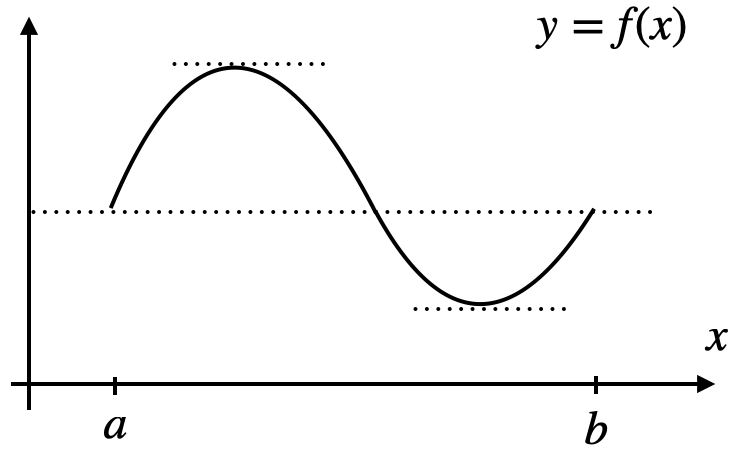
\includegraphics[width=50mm]{calculus8/Roll.png}
 \end{center}
\end{figure}

\end{frame}



%%%%%%%%%%%%%%%%%%%%%%%%%%%%%%%%%%%%%%%%%%%%%%%%%%%%%%%%%%%%%%%%%%%%%%%%%%%%%%%%%%%%%%%
%%%%%%%%%%%%%%%%%%%%%%%%%%%%%%%%%%%%%%%%%%%%%%%%%%%%%%%%%%%%%%%%%%%%%%%%%%%%%%%%%%%%%%%




\begin{frame}
\frametitle{平均値の定理(Mean Value theorem)}

ロルの定理を斜めにずらしたものが平均値の定理である. 

\begin{Thm}[平均値の定理]
微分可能な関数$f(x)$の定義域に$[a,b]$が含まれるとき,
$$
f'(c)=\frac{f(b)-f(a)}{b-a}
$$
を満たす$c \in (a,b)$が存在する. 
\end{Thm}

 \begin{figure}[htbp]
 \begin{center} 
  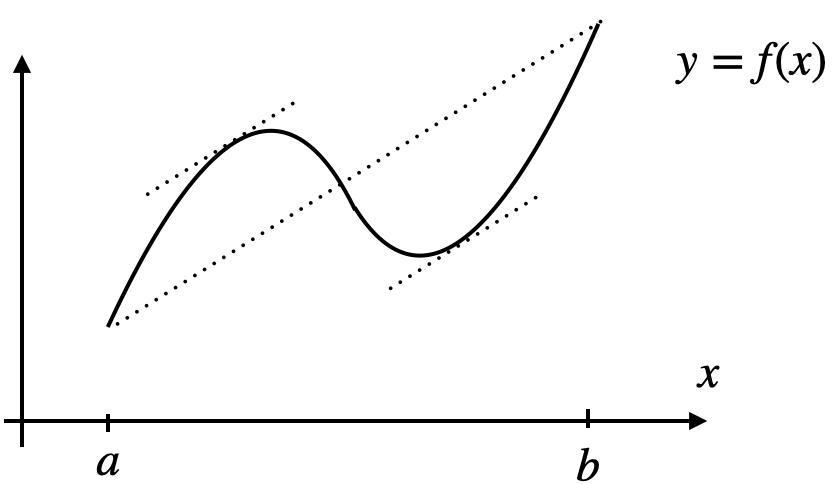
\includegraphics[width=50mm]{calculus8/Mean.png}
 \end{center}
\end{figure}

\end{frame}




%%%%%%%%%%%%%%%%%%%%%%%%%%%%%%%%%%%%%%%%%%%%%%%%%%%%%%%%%%%%%%%%%%%%%%%%%%%%%%%%%%%%%%%
%%%%%%%%%%%%%%%%%%%%%%%%%%%%%%%%%%%%%%%%%%%%%%%%%%%%%%%%%%%%%%%%%%%%%%%%%%%%%%%%%%%%%%%




\begin{frame}
\frametitle{平均値の定理の証明}


関数 
$$
g(x)=f(x)-\frac{f(b)-f(a)}{b-a}x
$$
は$g(a)=g(b)$を満たすので, ロルの定理より$g'(c)=0$なる$c \in (a,b)$が存在する. 
$$
0=g'(c)=f'(c)-\frac{f(b)-f(a)}{b-a}
$$
なので, 平均値の定理が示された. \\
\ \\

端点で関数の値が等しくなるように一次関数を引くことで, ロルの定理に帰着させている. 

\end{frame}



%%%%%%%%%%%%%%%%%%%%%%%%%%%%%%%%%%%%%%%%%%%%%%%%%%%%%%%%%%%%%%%%%%%%%%%%%%%%%%%%%%%%%%%
%%%%%%%%%%%%%%%%%%%%%%%%%%%%%%%%%%%%%%%%%%%%%%%%%%%%%%%%%%%%%%%%%%%%%%%%%%%%%%%%%%%%%%%




\begin{frame}
\frametitle{コーシーの平均値の定理}

\vspace{-1mm}

\begin{Thm}[コーシーの平均値の定理] 
微分可能な関数$f(x)$, $g(x)$の定義域に$[a,b]$が含まれ, $a<x<b$において$g'(x) \ne 0$であれば, 
$$
\frac{f(b)-f(a)}{g(b)-g(a)}=\frac{f'(c)}{g'(c)}
$$
なる$c \in (a,b)$が存在する. 
\end{Thm}

$g(x)=x$の場合が通常の平均値の定理である. 
直感的には媒介変数$t \in [a,b]$を用いて$(x,y)=(g(t),f(t))$の軌跡を考えれば良い. 

\vspace{-1mm}

 \begin{figure}[htbp]
 \begin{center} 
  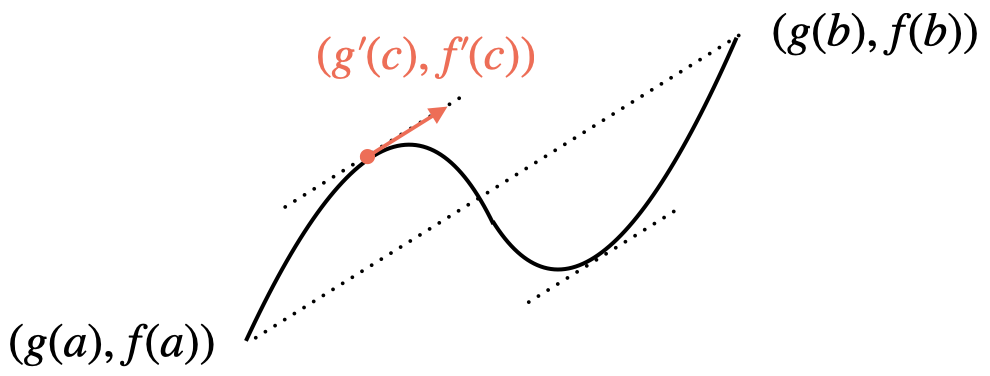
\includegraphics[width=60mm]{calculus8/CauchyMean.png}
 \end{center}
\end{figure}

\end{frame}




%%%%%%%%%%%%%%%%%%%%%%%%%%%%%%%%%%%%%%%%%%%%%%%%%%%%%%%%%%%%%%%%%%%%%%%%%%%%%%%%%%%%%%%
%%%%%%%%%%%%%%%%%%%%%%%%%%%%%%%%%%%%%%%%%%%%%%%%%%%%%%%%%%%%%%%%%%%%%%%%%%%%%%%%%%%%%%%



\begin{frame}
\frametitle{コーシーの平均値の定理の証明}

関数
$$
\phi(x)=\big(f(b)-f(a)\big)g(x)-\big(g(b)-g(a)\big)f(x)
$$
を考えると, 
$$
\phi(a)=g(a)f(b)-f(a)g(b)=\phi(b)
$$
であるから, ロルの定理より, ある$c \in (a,b)$が存在して
$$
0=\phi'(c)=\big(f(b)-f(a)\big)g'(c)-\big(g(b)-g(a)\big)f'(c). 
$$
一方で, ロルの定理の対偶を考えると$g'(c)\ne0$より$g(b)-g(a)\ne0$である. 
したがって, 上式を整理して
$$
\frac{f(b)-f(a)}{g(b)-g(a)}=\frac{f'(c)}{g'(c)}. 
$$



\end{frame}


%%%%%%%%%%%%%%%%%%%%%%%%%%%%%%%%%%%%%%%%%%%%%%%%%%%%%%%%%%%%%%%%%%%%%%%%%%%%%%%%%%%%%%%
%%%%%%%%%%%%%%%%%%%%%%%%%%%%%%%%%%%%%%%%%%%%%%%%%%%%%%%%%%%%%%%%%%%%%%%%%%%%%%%%%%%%%%%

\section{ロピタルの定理}

\begin{frame}
\frametitle{ロピタルの定理}

コーシーの平均値の定理を利用して, ロピタルの定理を証明する. 

\begin{Thm}[ロピタルの定理]
関数$f(x)$, $g(x)$が$a$を除く$a$の近傍において微分可能であり, 
$$
\lim_{x\to a}f(x) = \lim_{x\to a}g(x)=0
$$
かつ$g'(x) \ne0$とする. このとき極限$\displaystyle \lim_{x\to a}\frac{f'(x)}{g'(x)}$が存在するならば
$$
\lim_{x\to a}\frac{f(x)}{g(x)} = \lim_{x\to a}\frac{f'(x)}{g'(x)}. 
$$
\end{Thm}

ロピタルの定理は$a=\pm \infty$や$\displaystyle \lim_{x\to a}f(x) = \lim_{x\to a}g(x)=\pm \infty$の場合にも成立する. 

\end{frame}



%%%%%%%%%%%%%%%%%%%%%%%%%%%%%%%%%%%%%%%%%%%%%%%%%%%%%%%%%%%%%%%%%%%%%%%%%%%%%%%%%%%%%%%
%%%%%%%%%%%%%%%%%%%%%%%%%%%%%%%%%%%%%%%%%%%%%%%%%%%%%%%%%%%%%%%%%%%%%%%%%%%%%%%%%%%%%%%


\begin{frame}
\frametitle{ロピタルの定理の証明}
必要ならば$f(a)=g(a)=0$と置き直すことにより, $f(x)$, $g(x)$は点$a$を含めて連続としても極限には影響しない. \\
\ \\

$x>a$とすれば, $[a, x]$にコーシーの平均値の定理を適用して
$$
\frac{f(x)}{g(x)}=
\frac{f(x)-f(a)}{g(x)-g(a)}=
\frac{f'(c)}{g'(c)}
$$
なる$c \in (a,x)$が存在する. 
$x \to a+0$のとき$c \to a +0$であるから
$$
\lim_{x\to a+0}\frac{f(x)}{g(x)}  = \lim_{c \to a+0}\frac{f'(c)}{g'(c)}= \lim_{x\to a}\frac{f'(x)}{g'(x)}. 
$$
$x \to a-0$の場合も同様である. 

\end{frame}
\begin{slide}{ロピタルの定理の応用1}
次の極限を求めよ。
\begin{equation}
\lim_{x \to 0} \frac{\cos{x} - 1}{x^2} \nonumber
\end{equation}
\vspace{5mm}


分子 $\lim_{x\to0} \cos{x} - 1 = 0$, 分母 $\lim_{x\to 0}x^2 = 0$なので、分子、分母を微分して
\begin{equation}
\lim_{x \to 0} \frac{\cos{x} - 1}{x^2} = \lim_{x\to 0} \frac{-\sin{x}}{2x} \nonumber 
\end{equation}

この分子、分母の極限がどちらも0なのでさらに微分して
\begin{equation}
\lim_{x\to 0} \frac{-\sin{x}}{2x}=  \lim_{x\to 0} \frac{-\cos{x}}{2}=-\frac{1}{2}  \nonumber
\end{equation}


\end{slide}

\begin{slide}{ロピタルの定理の応用2}
次の極限を求めよ。
\begin{equation}
\lim_{x \to 0} x\log{x} \nonumber
\end{equation}
\vspace{5mm}


$\lim_{x\to 0} \log{x} = -\infty$なので
\begin{equation}
\lim_{x \to 0} x\log{x} = \lim_{x\to 0} \frac{\log{x}}{x^{-1}} \nonumber
\end{equation}
と変形すると分子はマイナス∞、 分母はプラス∞となる。分母分子を微分すると
\begin{equation}
\lim_{x\to 0} \frac{\log{x}}{x^{-1}}  = \lim_{x\to 0} \frac{\frac{1}{x}}{-x^{-2}}  = -\lim_{x\to 0} x = 0 \nonumber
\end{equation}

\end{slide}


\begin{slide}{ロピタルの定理の応用3}
次の極限を求めよ。
\begin{equation}
\lim_{x \to \infty} xe^{-x} \nonumber
\end{equation}
\vspace{5mm}


$\lim_{x\to \infty} x  = \infty$,  $\lim_{x\to \infty} e^{-x} = 0$なので
分母、分子を微分して
\begin{equation}
\lim_{x \to \infty} xe^{-x} = \lim_{x \to \infty}\frac{ 1}{e^{x}} = 0  \nonumber
\end{equation}


\end{slide}




%%%%%%%%%%%%%%%%%%%%%%%%%%%%%%%%%%%%%%%%%%%%%%%%%%%%%%%%%%%%%%%%%%%%%%%%%%%%%%%%%%%%%%%
%%%%%%%%%%%%%%%%%%%%%%%%%%%%%%%%%%%%%%%%%%%%%%%%%%%%%%%%%%%%%%%%%%%%%%%%%%%%%%%%%%%%%%%



\section{高次導関数}


\begin{frame}
\frametitle{高次導関数}


\begin{itemize}
\item 微分とは, 関数を$1$次多項式(関数)で近似した様子を記述するもの. 
導関数の情報から関数の増減の解析が可能になった. 
\item 導関数がさらに微分可能ならば, $2$回微分することにより凹凸を知ることができた. 
これは関数を$2$次多項式で近似することに相当する.
\item 関数がさらに微分可能の場合には, $3$回微分, $4$回微分, ... を考えることにより, 
与えられた関数の$3$次多項式, $4$次多項式, ... での近似を考察することができる. 
\end{itemize}


\end{frame}



%%%%%%%%%%%%%%%%%%%%%%%%%%%%%%%%%%%%%%%%%%%%%%%%%%%%%%%%%%%%%%%%%%%%%%%%%%%%%%%%%%%%%%%
%%%%%%%%%%%%%%%%%%%%%%%%%%%%%%%%%%%%%%%%%%%%%%%%%%%%%%%%%%%%%%%%%%%%%%%%%%%%%%%%%%%%%%%





\begin{frame}
\frametitle{高次導関数}


関数$f(x)$が微分可能なとき, $f'(x)$をその導関数と呼んだ. 
これを帰納的に繰り返すことで高次導関数を得ることができる. 
\begin{Def}
\begin{itemize}
\item $f'(x)$が微分可能なとき, $f^{(2)}(x)=f''(x)$を $f(x)$の\underline{$2$次導関数}という. 
\item $f^{(n-1)}(x)$が微分可能なとき, 
$$
f^{(n)}(x)=(f^{(n-1)}(x))'
$$
を$f(x)$の\underline{$n$次導関数}という. $\frac{d^n}{dx^n}f(x)$, $\frac{d^nf}{dx^n}(x)$とも書かれる.  
\end{itemize}
\end{Def}

記号を合わせるために, $f(x)$を$f^{(0)}(x)$, $f'(x)$を$f^{(1)}(x)$と書く場合もある.  


\end{frame}


%%%%%%%%%%%%%%%%%%%%%%%%%%%%%%%%%%%%%%%%%%%%%%%%%%%%%%%%%%%%%%%%%%%%%%%%%%%%%%%%%%%%%%%
%%%%%%%%%%%%%%%%%%%%%%%%%%%%%%%%%%%%%%%%%%%%%%%%%%%%%%%%%%%%%%%%%%%%%%%%%%%%%%%%%%%%%%%





\begin{frame}
\frametitle{高次導関数}


\begin{Def}
\begin{itemize}
\item 関数$f(x)$が$n$回微分可能であり, $f^{(n)}(x)$が連続であるとき, $f(x)$は$n$回連続微分可能, または$C^n$級であるという. 
\item 関数$f(x)$が何回でも微分可能であるとき, $f(x)$は無限回微分可能, または$C^\infty$級であるという. 
\end{itemize}
\end{Def}

\begin{itemize}
\item 実際の計算に現れる関数は$C^\infty$級であることが多いので, あまり神経質になる必要はない. 
\item 一方で, $f(x)=x^{\frac{1}{3}}$は微分可能であるが, $f'(x)=\frac{1}{3}x^{-\frac{2}{3}}$は原点$0$で連続でないため, $1$回連続微分可能でなはい. 
原点$0$以外では無限回微分可能である. 
\end{itemize}

\end{frame}




%%%%%%%%%%%%%%%%%%%%%%%%%%%%%%%%%%%%%%%%%%%%%%%%%%%%%%%%%%%%%%%%%%%%%%%%%%%%%%%%%%%%%%%
%%%%%%%%%%%%%%%%%%%%%%%%%%%%%%%%%%%%%%%%%%%%%%%%%%%%%%%%%%%%%%%%%%%%%%%%%%%%%%%%%%%%%%%





\begin{frame}
\frametitle{高次導関数}


$4$次多項式関数
$$
f(x)= 4x^4+6x^3-3x^2+7x-5
$$
に対して
\begin{align*}
f'(x) & = 16x^3+18x^2-6x+7, \\
f^{(2)}(x) & = 48x^2+36x-6, \\
f^{(3)}(x) & = 96x+36, \\
f^{(4)}(x) & = 96, \\
f^{(5)}(x) & = 0. 
\end{align*}


\end{frame}


%%%%%%%%%%%%%%%%%%%%%%%%%%%%%%%%%%%%%%%%%%%%%%%%%%%%%%%%%%%%%%%%%%%%%%%%%%%%%%%%%%%%%%%
%%%%%%%%%%%%%%%%%%%%%%%%%%%%%%%%%%%%%%%%%%%%%%%%%%%%%%%%%%%%%%%%%%%%%%%%%%%%%%%%%%%%%%%





\begin{frame}
\frametitle{高次導関数}

\begin{Prob}
次の関数の高次導関数を計算せよ. 
\begin{enumerate}
\item $\sin x$
\item $x^n$
\end{enumerate}
\end{Prob}


\end{frame}


%%%%%%%%%%%%%%%%%%%%%%%%%%%%%%%%%%%%%%%%%%%%%%%%%%%%%%%%%%%%%%%%%%%%%%%%%%%%%%%%%%%%%%%
%%%%%%%%%%%%%%%%%%%%%%%%%%%%%%%%%%%%%%%%%%%%%%%%%%%%%%%%%%%%%%%%%%%%%%%%%%%%%%%%%%%%%%%





\begin{frame}
\frametitle{$\sin x$の高次導関数}


$f(x)=\sin x$の高次導関数を計算する: 
\begin{align*}
f'(x) & = \cos x \\
f^{(2)}(x) & = -\sin x, \\
f^{(3)}(x) & = -\cos x \\
f^{(4)}(x) & =  \sin x
\end{align*}
であるから, 以下周期4でこれらを繰り返す. 
\end{frame}


%%%%%%%%%%%%%%%%%%%%%%%%%%%%%%%%%%%%%%%%%%%%%%%%%%%%%%%%%%%%%%%%%%%%%%%%%%%%%%%%%%%%%%%
%%%%%%%%%%%%%%%%%%%%%%%%%%%%%%%%%%%%%%%%%%%%%%%%%%%%%%%%%%%%%%%%%%%%%%%%%%%%%%%%%%%%%%%





\begin{frame}
\frametitle{$x^n$の高次導関数}


$f(x)=x^n$の高次導関数を計算する: 
\begin{align*}
f'(x) & = nx^{n-1} \\
f^{(2)}(x) & =n(n-1)x^{n-2}, \\
f^{(3)}(x) & = n(n-1)(n-2)x^{n-3}, \\
f^{(4)}(x) & =  n(n-1)(n-2)(n-3)x^{n-4}, \\
\dots & = \dots \\
f^{(n-1)}(x) & =  n(n-1)(n-2) \dots 2x, \\
f^{(n)}(x) & =  n(n-1)(n-2) \dots 2\cdot 1=n! 
\end{align*}
最後は$n$の階乗である. 
\end{frame}



%%%%%%%%%%%%%%%%%%%%%%%%%%%%%%%%%%%%%%%%%%%%%%%%%%%%%%%%%%%%%%%%%%%%%%%%%%%%%%%%%%%%%%%
%%%%%%%%%%%%%%%%%%%%%%%%%%%%%%%%%%%%%%%%%%%%%%%%%%%%%%%%%%%%%%%%%%%%%%%%%%%%%%%%%%%%%%%





\begin{frame}
\frametitle{多項式と高次導関数}


\begin{Thm} \label{多項式の係数}
$n$次多項式関数$f(x)$に関して
\begin{align*}
f(x) & = \sum_{k=0}^n\frac{f^{(k)}(0)}{k!}x^k \\
& =  f(0)+ f'(0)x + \frac{f^{(2)}(0)}{2!}x^2 +  \frac{f^{(3)}(0)}{3!}x^3+ \dots + \frac{f^{(n)}(0)}{n!}x^n. 
\end{align*}
ただし$0!=1$と定義した. 
\end{Thm}
つまり多項式$f(x)=a_0+a_1x+a_2x^2+\dots$に関して, $x^k$の係数は
$$
a_k=\frac{f^{(k)}(0)}{k!} 
$$
として計算できる. 

\end{frame}



%%%%%%%%%%%%%%%%%%%%%%%%%%%%%%%%%%%%%%%%%%%%%%%%%%%%%%%%%%%%%%%%%%%%%%%%%%%%%%%%%%%%%%%
%%%%%%%%%%%%%%%%%%%%%%%%%%%%%%%%%%%%%%%%%%%%%%%%%%%%%%%%%%%%%%%%%%%%%%%%%%%%%%%%%%%%%%%





\begin{frame}
\frametitle{定理\ref{多項式の係数}の証明}


多項式$f(x)=a_0+a_1x+a_2x^2+a_3x^3+\dots$に関して
\begin{align*}
f^{(1)}(x) &=a_1+2a_2x+3a_3x^2+4a_4x^3+\dots \\
f^{(2)}(x) &=2a_2+3\cdot 2 a_3x+4\cdot 3 a_4x^2+5\cdot 4 a_5 x^3+\dots \\
f^{(3)}(x) &=3\cdot 2 a_3+4\cdot 3 \cdot 2 a_4x+5\cdot 4 \cdot 3 a_5 x^2+\dots \\
\dots & = \dots \\ 
f^{(k)}(x) &= k! a_k +(k+1)\cdots 2a_{k+1}x+(k+2)\cdots 3a_{k+2}x^2+\dots
\end{align*}
であるから
$$
f^{(k)}(0)=k! a_k.  
$$

\end{frame}



%%%%%%%%%%%%%%%%%%%%%%%%%%%%%%%%%%%%%%%%%%%%%%%%%%%%%%%%%%%%%%%%%%%%%%%%%%%%%%%%%%%%%%%
%%%%%%%%%%%%%%%%%%%%%%%%%%%%%%%%%%%%%%%%%%%%%%%%%%%%%%%%%%%%%%%%%%%%%%%%%%%%%%%%%%%%%%%





\begin{frame}
\frametitle{多項式と高次導関数}

同様の議論で次も示すことができる. 

\begin{Thm} \label{poly_exp}
$n$次多項式関数$f(x)$に関して
\begin{align*}
f(x) & = \sum_{k=0}^n\frac{f^{(k)}(a)}{k!}(x-a)^k \\
& =  f(a)+ f'(a)(x-a) + \frac{f^{(2)}(a)}{2!}(x-a)^2  + \frac{f^{(3)}(a)}{3!}(x-a)^3 \\
& \ \ \ + \dots + \frac{f^{(n)}(a)}{n!}(x-a)^n. 
\end{align*}
\end{Thm}


\end{frame}


%%%%%%%%%%%%%%%%%%%%%%%%%%%%%%%%%%%%%%%%%%%%%%%%%%%%%%%%%%%%%%%%%%%%%%%%%%%%%%%%%%%%%%%
%%%%%%%%%%%%%%%%%%%%%%%%%%%%%%%%%%%%%%%%%%%%%%%%%%%%%%%%%%%%%%%%%%%%%%%%%%%%%%%%%%%%%%%





\begin{frame}
\frametitle{多項式と高次導関数}

$f(x)= 4x^4+6x^3-3x^2+7x-5$に関して
\begin{align*}
f'(x) & = 16x^3+18x^2-6x+7, \ \ \ f^{(2)}(x)  = 48x^2+36x-6, \\
f^{(3)}(x) & = 96x+36, \ \ \ f^{(4)}(x)  = 96. 
\end{align*}
これより, 次はどちらも$f(x)$に一致する. 
\begin{align*}
&  f(0)+ f'(0)x + \frac{f^{(2)}(0)}{2!}x^2  + \frac{f^{(3)}(0)}{3!}x^3+  \frac{f^{(4)}(0)}{4!}x^4 \\
& \ \ \ = -5 + 7x + \frac{-6}{2}x^2+\frac{36}{6}x^3+\frac{96}{24}x^4 \\
&  f(1)+ f'(1)(x-1) + \frac{f^{(2)}(1)}{2!}(x-1)^2  + \frac{f^{(3)}(1)}{3!}(x-1)^3+  \frac{f^{(4)}(1)}{4!}(x-1)^4 \\
& \ \ \ = 9 + 35(x-1) + \frac{78}{2}(x-1)^2+\frac{132}{6}(x-1)^3+\frac{96}{24}(x-1)^4 
\end{align*}

\end{frame}


%%%%%%%%%%%%%%%%%%%%%%%%%%%%%%%%%%%%%%%%%%%%%%%%%%%%%%%%%%%%%%%%%%%%%%%%%%%%%%%%%%%%%%%
%%%%%%%%%%%%%%%%%%%%%%%%%%%%%%%%%%%%%%%%%%%%%%%%%%%%%%%%%%%%%%%%%%%%%%%%%%%%%%%%%%%%%%%





\begin{frame}
\frametitle{多項式と高次導関数}

\begin{Prob}
定理\ref{poly_exp}を, 関数$f(x)=3x^2-x+5$と$a=0,\pm1$に関して確認せよ. つまり
\begin{align*}
f(x) & = f(0)+ f'(0)x + \frac{f^{(2)}(0)}{2!}x^2 \\
f(x) & = f(1)+ f'(1)(x-1) + \frac{f^{(2)}(1)}{2!}(x-1)^2 \\
f(x) & = f(-1)+ f'(-1)(x+1) + \frac{f^{(2)}(-1)}{2!}(x+1)^2 
\end{align*}
が成立することを確認せよ. 
\end{Prob}


\end{frame}
%%%%%%%%%%%%%%%%%%%%%%%%%%%%%%%%%%%%%%%%%%%%%%%%%%%%%%%%%%%%%%%%%%%%%%%%%%%%%%%%%%%%%%%
%%%%%%%%%%%%%%%%%%%%%%%%%%%%%%%%%%%%%%%%%%%%%%%%%%%%%%%%%%%%%%%%%%%%%%%%%%%%%%%%%%%%%%%

\section{テイラーの定理}

\begin{frame}

\frametitle{平均値の定理}


平均値の定理を思い出す. 
\begin{Thm}[平均値の定理]
微分可能な関数$f(x)$の定義域に$[a,b]$が含まれるとき, %\vspace{-2mm}
$$
f'(c)=\frac{f(b)-f(a)}{b-a}
$$
を満たす$c \in (a,b)$が存在する. 
\end{Thm}

上記の式は, 次と同値
$$
f(b)=f(a)+f'(c)(b-a) \ \ \ (c \in (a,b)). 
$$
高次導関数を用いて, 平均値の定理はテイラーの定理に一般化される. 

\end{frame}




%%%%%%%%%%%%%%%%%%%%%%%%%%%%%%%%%%%%%%%%%%%%%%%%%%%%%%%%%%%%%%%%%%%%%%%%%%%%%%%%%%%%%%%
%%%%%%%%%%%%%%%%%%%%%%%%%%%%%%%%%%%%%%%%%%%%%%%%%%%%%%%%%%%%%%%%%%%%%%%%%%%%%%%%%%%%%%%



\begin{frame}
\frametitle{テイラーの定理}


\begin{Thm}[テイラーの定理] \label{テイラー}
開区間$I$で定義された関数$f(x)$が$n$回微分可能であるとき. 
任意の$a \in I$に対して, 
 \begin{align*}
f(x) & = \sum_{k=0}^{n-1}\frac{f^{(k)}(a)}{k!}(x-a)^k + \frac{f^{(n)}(c)}{k!}(x-a)^n \\
& =  f(a)+ f'(a)(x-a) + \frac{f^{(2)}(a)}{2!}(x-a)^2  + \frac{f^{(3)}(a)}{3!}(x-a)^3 \\
& \ \ \ + \dots + \frac{f^{(n-1)}(a)}{(n-1)!}(x-a)^{n-1}+\frac{f^{(n)}(c)}{n!}(x-a)^n . 
\end{align*}
を満たす$c \in (a,x)$が存在する. ($a<x$の場合) 
\end{Thm}
上記の表示を有限テイラー展開という. 
証明は次回. 


\end{frame}





%%%%%%%%%%%%%%%%%%%%%%%%%%%%%%%%%%%%%%%%%%%%%%%%%%%%%%%%%%%%%%%%%%%%%%%%%%%%%%%%%%%%%%%
%%%%%%%%%%%%%%%%%%%%%%%%%%%%%%%%%%%%%%%%%%%%%%%%%%%%%%%%%%%%%%%%%%%%%%%%%%%%%%%%%%%%%%%



\begin{frame}
\frametitle{マクローリンの定理}


特に$a=0$の場合にはマクローリンの定理と呼ばれる. 


\begin{Thm}[マクローリンの定理]  \label{マクローリン}
$0$を含む開区間$I$で定義された関数$f(x)$が$n$回微分可能であるとき. 
 \begin{align*}
f(x) & = \sum_{k=0}^{n-1}\frac{f^{(k)}(0)}{k!}x^k + \frac{f^{(n)}(\theta x)}{n!}x^n \\
& =  f(0)+ f'(0)x + \frac{f^{(2)}(0)}{2!}x^2  + \frac{f^{(3)}(0)}{3!}x^3 \\
& \ \ \ + \dots + \frac{f^{(n-1)}(0)}{(n-1)!}x^{n-1}+\frac{f^{(n)}(\theta x)}{n!}x^n . 
\end{align*}
を満たす$\theta \in (0,1)$が存在する. ($0<x$の場合) 
\end{Thm}
上記の表示を有限マクローリン展開という.

\end{frame}


%%%%%%%%%%%%%%%%%%%%%%%%%%%%%%%%%%%%%%%%%%%%%%%%%%%%%%%%%%%%%%%%%%%%%%%%%%%%%%%%%%%%%%%
%%%%%%%%%%%%%%%%%%%%%%%%%%%%%%%%%%%%%%%%%%%%%%%%%%%%%%%%%%%%%%%%%%%%%%%%%%%%%%%%%%%%%%%



\begin{frame}
\frametitle{テイラーの定理}


\begin{itemize}
\item テイラーの定理における
$$
P_{n-1}(x)=\sum_{k=0}^{n-1}\frac{f^{(k)}(a)}{k!}(x-a)^k, \ \ \ 
R_n(x)=\frac{f^{(n)}(c)}{k!}(x-a)^n
$$
はそれぞれ($n-1$次の)\underline{テイラー多項式}と\underline{剰余項}と呼ばれる. 
\item 微分の観点からは, $f(x)$と$P_{n-1}(x)$は似ている. 
$$
f(a)=P_{n-1}(a), \ \ f '(a)=P'_{n-1}(a), \ \dots, \  f^{(n-1)}(a)=P^{(n-1)}_{n-1}(a). 
$$
実際, $f(x)$が$n$次多項式であれば, $f(x)=P_n(x)$であった. 
\item テイラーの定理は$f(x)$と$P_{n-1}(x)$の誤差を$f(x)$の$n$次微分係数を用いて評価できることを主張している. 
\end{itemize}

\end{frame}



%%%%%%%%%%%%%%%%%%%%%%%%%%%%%%%%%%%%%%%%%%%%%%%%%%%%%%%%%%%%%%%%%%%%%%%%%%%%%%%%%%%%%%%
%%%%%%%%%%%%%%%%%%%%%%%%%%%%%%%%%%%%%%%%%%%%%%%%%%%%%%%%%%%%%%%%%%%%%%%%%%%%%%%%%%%%%%%



\begin{frame}
\frametitle{$e^x$の有限マクローリン展開}

$f(x)=e^x$の有限マクローリン展開を求める. 
$$
f'(x)=f^{(2)}(x)=f^{(3)}(x)=f^{(4)}(x)=e^x
$$
であるから
$$
f'(0)=f^{(2)}(0)=f^{(3)}(0)=f^{(4)}(0)=e^0=1. 
$$
したがって
\begin{align*}
e^x &= P_5(x)+R_6(x) \\
& = 1+x+\frac{x^2}{2!}+\frac{x^3}{3!}+\frac{x^4}{4!}+\frac{x^5}{5!}+\frac{e^{\theta x}}{6!}x^6. 
\end{align*}

\end{frame}



%%%%%%%%%%%%%%%%%%%%%%%%%%%%%%%%%%%%%%%%%%%%%%%%%%%%%%%%%%%%%%%%%%%%%%%%%%%%%%%%%%%%%%%
%%%%%%%%%%%%%%%%%%%%%%%%%%%%%%%%%%%%%%%%%%%%%%%%%%%%%%%%%%%%%%%%%%%%%%%%%%%%%%%%%%%%%%%



\begin{frame}
\frametitle{$e^x$の有限マクローリン展開}

$f(x)=e^x$の有限マクローリン展開
\begin{align*}
e^x &= P_5(x)+R_6(x) \\
& = 1+x+\frac{x^2}{2!}+\frac{x^3}{3!}+\frac{x^4}{4!}+\frac{x^5}{5!}+\frac{e^{\theta x}}{6!}x^6. 
\end{align*}
を用いて$f(1)=e$の近似値を求める. 
$$
P_5(1)=\frac{163}{60}=2.71666\dots
$$
であるが, マクローリンの定理より誤差は, $e<3$を知っていれば, 
$$
|e-P_5(1)|=\frac{e^\theta}{6!}<\frac{e}{6!}<\frac{3}{6!}=\frac{1}{240}=0.004166\dots
$$

\end{frame}



%%%%%%%%%%%%%%%%%%%%%%%%%%%%%%%%%%%%%%%%%%%%%%%%%%%%%%%%%%%%%%%%%%%%%%%%%%%%%%%%%%%%%%%
%%%%%%%%%%%%%%%%%%%%%%%%%%%%%%%%%%%%%%%%%%%%%%%%%%%%%%%%%%%%%%%%%%%%%%%%%%%%%%%%%%%%%%%



\begin{frame}
\frametitle{$\sin x$有限のマクローリン展開}

$f(x)=\sin x$の有限マクローリン展開を求める. 
$$
f'(x)=\cos x, \ f^{(2)}(x)=-\sin x, \ f^{(3)}(x)=-\cos x, \ f^{(4)}(x)=\sin x
$$
を周期$4$で繰り返すことから
$$
 f^{(4n)}(0)=0, \ f^{(4n+1)}(0)=1, \ f^{(4n+2)}(0)=0, \ f^{(4n+3)}(0)=-1. 
$$
したがって
$$
\sin x =x-\frac{x^3}{3!}+\frac{x^5}{5!}+R_7(x)
$$
ここで
$$
R_7(x)=- \frac{\cos (\theta x)}{7!}x^7 \ \ \ (0 < \theta <1)
$$
ただし$P_5(x)=P_6(x)$に注意する. 
\end{frame}


%%%%%%%%%%%%%%%%%%%%%%%%%%%%%%%%%%%%%%%%%%%%%%%%%%%%%%%%%%%%%%%%%%%%%%%%%%%%%%%%%%%%%%%
%%%%%%%%%%%%%%%%%%%%%%%%%%%%%%%%%%%%%%%%%%%%%%%%%%%%%%%%%%%%%%%%%%%%%%%%%%%%%%%%%%%%%%%


\begin{frame}
\frametitle{昇ベキと降ベキ}

\begin{itemize}
\item 多項式を書くとき, 通常は次数が高い方から書くことが多い. 例えば
$$
5x^3-x^2+5x-10. 
$$
このような表示を\underline{降ベキ}の順という. 
\item 一方で, (有限)マクローリン展開などを議論するときは次数が低い方から書くことが多い. 例えば
$$
-10+5x-x^2+5x^3. 
$$
このような表示を\underline{昇ベキ}の順という. 
\end{itemize}

$x$が一般の場合には降ベキ, $x$が十分小さい場合には昇ベキを使うことが多い. 

\end{frame}




%%%%%%%%%%%%%%%%%%%%%%%%%%%%%%%%%%%%%%%%%%%%%%%%%%%%%%%%%%%%%%%%%%%%%%%%%%%%%%%%%%%%%%%
%%%%%%%%%%%%%%%%%%%%%%%%%%%%%%%%%%%%%%%%%%%%%%%%%%%%%%%%%%%%%%%%%%%%%%%%%%%%%%%%%%%%%%%





%%%%%%%%%%%%%%%%%%%%%%%%%%%%%%%%%%%%%%%%%%%%%%%%%%%%%%%%%%%%%%%%%%%%%%%%%%%%%%%%%%%%%%%
%%%%%%%%%%%%%%%%%%%%%%%%%%%%%%%%%%%%%%%%%%%%%%%%%%%%%%%%%%%%%%%%%%%%%%%%%%%%%%%%%%%%%%%




\section{今日のまとめ}
\begin{frame}
\frametitle{まとめ}   


\begin{enumerate}
\item ロルの定理, 平均値の定理, コーシーの平均値の定理, 
\item 高次導関数, テイラーの定理, 有限テイラー展開
\end{enumerate} 

\end{frame}